\documentclass{article}
\usepackage{xcolor}
\usepackage{amsmath}
\usepackage{amsfonts}
\begin{document}
\textbf{1169. (\color{red}d0\color{black}, Unknown)} In a distant country there are 2 cities, City $A$ and City $B$, which are $40$ kilometers apart.  $2000$ students live in City $A$, and $1000$ live in City $B$. Where should the government build the school which all students from both cities will attend, so that the sum of the necessary walking distance of all the students will be minimal?

\textbf{1036. (\color{red}d0\color{black}, 2017 AIME I, P1 of 15)} Fifteen distinct points are designated on $\triangle ABC$: the 3 vertices $A$, $B$, and $C$; $3$ other points on side $\overline{AB}$; $4$ other points on side $\overline{BC}$; and $5$ other points on side $\overline{CA}$. Find the number of triangles with positive area whose vertices are among these $15$ points.

\textbf{924. (\color{red}d1\color{black}, PST 16.2.3)} Given \(n\) points in the plane, no three of which are collinear, show it is possible to join them up
in a sequence so that we have a broken line consisting of \(n-1\) segments, no two of which cross
each other.

\textbf{917. (\color{red}d1\color{black}, Folklore)} There are \(n\) students standing in a field such that the distance between each pair is distinct. Each student is holding a ball, and when the teacher blows a whistle, each student throws their ball to the nearest student. Prove that there is a pair of students that throw their balls to each other.

\textbf{861. (\color{red}d1\color{black}, 2002 Putnam, A2)} Show that, whenever five dots are drawn on a sphere, the sphere can be cut in half in such a way that four of the points are on the same half.

\textbf{756. (\color{red}d1\color{black}, PST 14.0.7)} A \emph{snozzberry} has the shape of a convex polyhedron such that three faces meet at every vertex, and each face is either a pentagon or a hexagon. Each pentagon is surrounded by five hexagons while each hexagon is surrounded by three hexagons and three pentagons.

\vspace{0.75em}

How many faces does a snozzberry have?

\textbf{638. (\color{red}d1\color{black}, 2019 UK JMO, B6)} An equilateral triangle is divided into smaller equilateral triangles.

\begin{center}
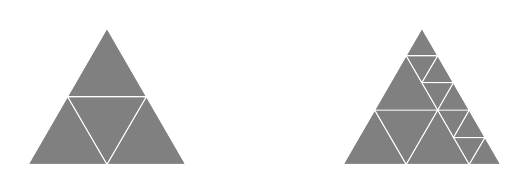
\begin{tikzpicture}
\fill [gray] (0,0) -- (1, 1.73) -- (2,0) -- (0,0);
\draw [white] (0,0) -- (1, 1.73) -- (2,0) -- (0,0);
\draw [white] (0.5, 0.86) -- (1.5,0.86) -- (1,0) -- (0.5, 0.86);

\fill [gray] (4,0) -- (5, 1.73) -- (6,0) -- (4,0);
\draw [white] (4,0) -- (5, 1.73) -- (6,0) -- (4,0);
\draw [white] (4.4, 0.69) -- (4.8, 0) -- (5.2, 0.69) -- (4.4, 0.69);
\draw [white] (4.8, 1.38) -- (5.6, 0);
\draw [white] (4.8, 1.38) -- (5.2, 1.38) -- (5, 1.04) -- (5.4, 1.04) -- (5.2, 0.69) -- (5.6, 0.69) -- (5.4, 0.34) -- (5.8, 0.34) -- (5.6, 0);
\end{tikzpicture}
\end{center}

The diagram on the left shows that it is possible to divide it into 4 equilateral triangles.

The diagram on the right shows that it is possible to divide it into 13 equilateral triangles.

What are the integer values of $n$, where $n>1$, for which it is possible to divide the triangle into $n$ smaller equilateral triangles?

\textbf{1260. (\color{red}d2\color{black}, 2013 Chile Classification NMO, P1 of 6)} Ten points are chosen inside an equilateral triangle of side 4. Show that there are two chosen points at distance at most $\sqrt{3}$.

\textbf{1212. (\color{red}d2\color{black}, 2017 UK SMC, P24 of 25, adapted)} There is a set of straight lines in the plane such that each line intersects exactly ten others. What are the possible values for the number of lines in the set?

\textbf{1072. (\color{red}d2\color{black}, 2021–22 ICMC, Round 2, P1 of 5)} Let $S$ be a set of 2022 lines in the plane, no two parallel, no three concurrent. $S$ divides the plane into finite regions and infinite regions. Is it possible for all the finite regions to have integer area?

\textbf{883. (\color{red}d2\color{black}, Folklore)} Tony Wang has an infinite piece of paper and he draws $n$ infinite lines on it, none of which are parallel. Suppose also that no three lines meet at one point. How many points are there that are where two lines intersect? How many regions has he divided his piece of paper into?

\textbf{666. (\color{red}d2\color{black}, Problems in Plane and Solid Geometry, Problem 21.10)} What is the least number of points one has to mark inside a convex $n$-gon in order for the interior of any triangle with the vertices at vertices of the $n$-gon to contain at least one of the marked points?

\textbf{518. (\color{red}d2\color{black}, 2020 OMO Spring, Q6 of 30)} Alexis has 2020 paintings, the $i$th one of which is a $1 \times i$ rectangle for $i=1,2, \ldots, 2020 .$ Compute the smallest integer $n$ for which they can place all of the paintings onto an $n \times n$ mahogany table without overlapping or hanging off the table.

\textbf{154. (\color{red}d2\color{black}, 2009 Putnam, A1)} Let $f$ be a real-valued function on the plane such that for every square $ABCD$ in the plane, $f(A) + f(B) + f(C) +f(D) = 0$. Does it follow that $f(P) = 0$ for all points $P$ in the plane?

\textbf{148. (\color{red}d2\color{black}, 2015 ToT Senior O-Level Paper, P2 of 5)} A moth made four small holes in a square carpet with a 275 cm side. Can one

always cut out a square piece with a 1m side without holes? (Consider holes

as points). 

\textbf{76. (\color{red}d2\color{black}, 2006 Irish MO (19th), Part I, Q3 of 5)} Prove that a square of side 2.1 units can be completely covered by seven squares of side 1 unit.

\textbf{59. (\color{red}d2\color{black}, 2019 New Zealand Squad Selection Test, Q2 of 8)} Andrew chooses a set $A$ of 100 different points in the plane, no three of them collinear. Show that amongst the triangles with all their vertices in $A$, there are at least 100 that are not equilateral.

\textbf{1101. (\color{red}d3\color{black}, 2019 CHMMC P3 of 10)} A frog is jumping between lattice points on the coordinate plane in the following way: On each jump, the frog randomly goes to one of the 8 closest lattice points to it, such that the frog never goes in the same direction on consecutive jumps. If the frog starts at $(20, 19)$ and jumps to $(20, 20)$, then what is the expected value of the frog's position after it jumps for an infinitely long time?

\textbf{680. (\color{red}d3\color{black}, Folklore)} Define an $n$-collection to be an arrangement of $n$ points in the plane such that no three are collinear and each is colored either red or blue. What is the smallest value of $n$ such that in any $n$-collection, there will always exist two monochromatic triangles (triangles having either all blue points or all red points as vertices) which do not intersect?

\textbf{660. (\color{red}d3\color{black}, 2020 ICMC Round 1, P1 of 6)} A set of points in the plane is called \emph{sane} if no three points are collinear and the angle between any three distinct points is a rational number of degrees.

a) Does there exist a countably infinite sane set $\mathcal{P}$?

b) Does there exist an uncountably infinite sane set $\mathcal{Q}$?

\emph{Note: a set S is countable if there exists a bijection between S and the natural numbers.}

\textbf{317. (\color{red}d3\color{black}, The coin game (ACPS, 3.1.20))} Consider the following two-player game. Each player takes turns placing a penny on the surface of a rectangular table. No penny can touch a penny that is already on the table. The table starts out with no pennies. The last player who makes a legal move wins. Does the first player have a winning strategy?

\textbf{290. (\color{red}d3\color{black}, 2020 ICMC, Round 1, P1 of 6)} Alice and Bob play a game on a sphere which is initially marked with a finite number of points. Alice and Bob then take turns making moves, with Alice going first:

\begin{itemize}

\item On Alice's move, she counts the number of marked points on the sphere, $ n $. She then marks another $ n + 1 $ points on the sphere.

\item On Bob's move, he chooses one hemisphere and removes all marked points on that hemisphere, including any marked points on the boundary of the hemisphere.

\end{itemize}

Can Bob always guarantee that after a finite number of moves, the sphere contains no marked points?



(A \emph{hemisphere} is the region on a sphere that lies completely on one side of any plane passing through the centre of the sphere.)

\textbf{103. (\color{red}d3\color{black}, 2019 AMO, Q4)} Let \(Q\) be a point inside the convex polygon \(P_1 P_2 \dots P_{1000}\). For each \(i=1, 2, \dots, 1000\), extend the line \(P_i Q\) until it meets the polygon again at a point \(X_i\). Suppose that one of the points \(X_1, X_2, \dots, X_{1000}\) is a vertex of the polygon.\\
\makebox[16pt]{}Prove that there is at least one side of the polygon that does not contain any of the points \(X_1, X_2, \dots, X_{1000}\).

\textbf{94. (\color{red}d3\color{black}, 2007 Mongolian MO Secondary, Q2)} Given 101 segments on a line, prove that there either exists a point contained in at least 11 of the segments, or at least 11 segments that are pairwise disjoint.

\textbf{48. (\color{red}d3\color{black}, 2009 Canada MO, Q5 of 5)} A set of points is marked on the plane, with the property that any three marked points can be covered with a disk of radius 1. Prove that the set of all marked points can be covered with a disk of radius 1.

\textbf{1353. (\color{red}d4\color{black}, 2023 BMO1, P6 of 6)} A circle $\Gamma$ has radius 1. A line $\ell$ is such that the perpendicular distance from $\ell$ to the centre of $\Gamma$ is strictly between 0 and 2. A frog chooses a point on $\Gamma$ whose perpendicular distance from $\ell$ is less than 1 and sits on a point. It then performs a sequence of jumps. Each jump has length 1 and if a jump starts on $\Gamma$ it must end on $\ell$ and vice versa. Prove that after some finite number of jumps the frog returns to a point it has been on before.

\textbf{1199. (\color{red}d4\color{black}, 2021 USAMTS R3 P3 of 5)} Sydney the squirrel is at $(0, 0)$ and is trying to get to $(2021, 2022).$ She can move only by reflecting her position over any line that can be formed by connecting two lattice points, provided that the reflection puts her on another lattice point. Is it possible for Sydney to reach $(2021, 2022)$?


\textbf{1031. (\color{red}d4\color{black}, 2008 USAMO, P4 of 6)} Let $\mathcal{P}$ be a convex polygon with $n$ sides, $n\ge3$. Any set of $n-3$ diagonals of $\mathcal{P}$ that do not intersect in the interior of the polygon determine a triangulation of $\mathcal{P}$ into $n - 2$ triangles. If $\mathcal{P}$ is regular and there is a triangulation of $\mathcal{P}$ consisting of only isosceles triangles, find all the possible values of $n$.

\textbf{731. (\color{red}d4\color{black}, Coffin Problems)} The plane is coloured into three different colours. Prove that there exist two points of the same color with a given distance between them.

\textbf{702. (\color{red}d4\color{black}, 2020 CHMMC Proof P4)} Fix a positive integer $n$. Pick $4n$ equally spaced points on a circle and color them alternately
blue and red. You use $n$ blue chords to pair the $2n$ blue points, and you use $n$ red chords to pair
the $2n$ red points. If some blue chord intersects some other red chord, then such a pair of chords
is called a “good pair."  Find, with proof, the minimum number of good pairs
under all possible configurations of chord pairings.

\textbf{521. (\color{red}d4\color{black}, 2016 AMO, P7 of 8)} Each point in the plane is assigned one of four colours.

Prove that there exist two points at distance $1$ or $\sqrt3$ from each other that are assigned the same colour.

\textbf{323. (\color{red}d4\color{black}, 1991 APMO, P2 of 5)} There are 997 points in the plane. Show that they have at least 1991 distinct midpoints. Is it possible to have exactly 1991 midpoints?

\textbf{203. (\color{red}d4\color{black}, Christmas Junior MO, P1 of 6)} Call a convex equilateral polygon $\textit{rhomboidal}$ if it can be tiled with a finite number of non-overlapping rhombi that have the same side length of the polygon. Prove that a convex equilateral polygon is $\textit{rhomboidal}$ if and only if each side of the polygon is parallel to some other side of the polygon.

\textbf{112. (\color{red}d4\color{black}, 2018 Canadian MO, P1)} Consider an arrangement of tokens in the plane, not necessarily at distinct points. We are allowed to apply a sequence of moves of the following kind: Select a pair of tokens at points A and B and move both of them to the midpoint of A and B.\\
We say that an arrangement of \(n\) tokens is \textit{collapsible} if it is possible to end up with all \(n\) tokens at the same point after a finite number of moves. Prove that every arrangement of \(n\) tokens is collapsible if and only if \(n\) is a power of 2.

\textbf{89. (\color{red}d4\color{black}, 2018 NZ Camp Selection Problems, Q6)} The intersection of a cube and a plane is a pentagon. Prove that the length of at least one side of the pentagon differs from 1 metre by at least 20 centimetres. 

\textbf{1179. (\color{red}d5\color{black}, 2022 Malaysia IMO TST, P2 of 6)} Let $\mathcal{S}$ be a set of $2023$ points in a plane, and it is known that the distances of any two different points in $S$ are all distinct. Ivan colors the points with $k$ colors such that for every point $P \in \mathcal{S}$, the closest and the furthest point from $P$ in $\mathcal{S}$ also have the same color as $P$.

What is the maximum possible value of $k$?

\textbf{1150. (\color{red}d5\color{black}, 2018 CMO, P1 of 5)} Consider an arrangement of tokens in the plane, not necessarily at distinct points. We are allowed
to apply a sequence of moves of the following kind: Select a pair of tokens at points $A$ and $B$ and
move both of them to the midpoint of $A$ and $B$.

We say that an arrangement of $n$ tokens is $collapsible$ if it is possible to end up with all $n$ tokens at
the same point after a finite number of moves. Prove that every arrangement of $n$ tokens is
collapsible if and only if $n$ is a power of 2.

\textbf{695. (\color{red}d5\color{black}, OTIS Anti-Problems)} A \emph{diamond} is a rhombus with side length 1 whose interior angles are $60^{\circ}$ and $120^{\circ}$ (hence with area $\sqrt{3}/2$). A regular hexagon $\mathcal{H}$ of side length $10$ is dissected into diamonds. In a move, if three pairwise adjacent diamonds form a regular hexagon of side length $1$, one may rotate all three $60^{\circ}$ about the center of that hexagon. Find the smallest positive integer $N$ such that any tiling of $\mathcal{H}$ can be transformed into any other in at most $N$ moves, or show that no such $N$ exists.

\textbf{654. (\color{red}d5\color{black}, 2019 IGO Advanced, P2 of 5)} Is it true that in any convex $n$-gon with $n > 3$, there exists a vertex and a diagonal passing through this vertex such that the angles of this diagonal with both sides adjacent to this vertex are acute?

\textbf{583. (\color{red}d5\color{black}, 2020 Hong Kong TST 2, P2 of 4)} Suppose there are $2019$ distinct points in a plane and the distances between pairs of them attain $k$ different values. Prove that $k$ is at least $44$.

\textbf{465. (\color{red}d5\color{black}, 2017 AMO, P4 of 8)} Suppose that $S$ is a set of 2017 points in the plane that are not all collinear.

Prove that $S$ contains three points that form a triangle whose circumcentre is not a point in $S$.

\textbf{157. (\color{red}d5\color{black}, IGO 2017 Senior, P2 of 5)} We have six pairwise non-intersecting circles that the radius of each is at least one. Prove that the radius of any circle intersecting all the six circles, is at least one.

\textbf{1278. (\color{red}d6\color{black}, nan)} Tony Wang's arch-nemesis, Bony Wang, has laid out some bowls on the floor and made some really long noodles which stretch between different bowls. He places these noodles in the bowls so that each noodle has its ends in different bowls. In an attempt to avoid dying, Bony has been careful not to make it appear that any two noodles cross if you look at this masterpiece from above. Bony challenges Tony to fill every bowl with Chinese Noodle Soup in such a way that no two bowls which share one of Bony's noodles are filled with the same flavour of Chinese Noodle Soup. However, Tony only knows how to make five different flavours of Chinese Noodle Soup (and no mixing is allowed)! Show that Tony can still manage this task.

\textbf{1172. (\color{red}d6\color{black}, 2021 Sharygin Geometry Olympiad, Final Round, Day 1, 9 Form, P4 of 8)} Define the \emph{distance} between two triangles to be the closest distance between two vertices, one from each triangle. Is it possible to draw five triangles in the plane such that for any two of them, their distance equals the sum of their circumradii?

\textbf{969. (\color{red}d6\color{black}, 2018 RMMSL, C1)} Call a point in the Cartesian plane with integer coordinates a \textit{lattice point}. Given a finite set $\mathcal{S}$ of lattice points we repeatedly perform the following operation: given two distinct lattice points $A, B$ in $\mathcal{S}$ and two distinct lattice points $C, D$ not in $\mathcal{S}$ such that $ACBD$ is a parallelogram with $AB > CD$, we replace $A, B$ by $C, D$. Show that only finitely many such operations can be performed.

\textbf{809. (\color{red}d6\color{black}, Inaba's Theorem)} Prove that any set of 10 points in the plane ($\mathbb{R}^2$) can be covered by a suitable placement of disjoint open unit disks.

\textbf{620. (\color{red}d6\color{black}, 2018 IMOSL, G3)} A circle $\omega$ with radius $1$ is given. A collection $T$ of triangles is called good, if the following conditions hold:

    each triangle from $T$ is inscribed in $\omega$;
    no two triangles from $T$ have a common interior point.

Determine all positive real numbers $t$ such that, for each positive integer $n$, there exists a good collection of $n$ triangles, each of perimeter greater than $t$.

\textbf{541. (\color{red}d6\color{black}, 1990 IMO, P6 of 6)} Prove that there exists a convex 1990-gon with the following two properties :
\smallbreak
a.) All angles are equal.
\smallbreak
b.) The lengths of the 1990 sides are the numbers $ 1^2$, $ 2^2$, $ 3^2$, $ \cdots$, $ 1990^2$ in some order.

\textbf{220. (\color{red}d6\color{black}, 2018 ICL-plus)} Suppose that we can cover a triangle using 100 (possibly overlapping) circles of radius 2. Prove that we can cover it using 493 circles of radius 1.

\textbf{102. (\color{red}d6\color{black}, 2013 IMO Shortlist, C2)} In the plane, 2013 red points and 2014 blue points are marked so that no three of the marked points are collinear. One needs to draw \(k\) lines not passing through the marked points and dividing the plane into several regions. The goal is to do it in such a way that no region contains points of both colors.\\

Find the minimal value of \(k\) such that the goal is attainable for every possible configuration of 4027 points.

\textbf{1118. (\color{red}d7\color{black}, 2022 DAMO, P1 of 6)} 101 distinct rays lie on a plane. No two rays share an endpoint or coincide, and no three rays concur. Find the maximum number of unordered pairs $(a, b) $ of rays such that $a$ and $b$ intersect at a point $C$ which is equidistant from the endpoints of $a$ and $b$. 

\textbf{795. (\color{red}d7\color{black}, 2021 Irish MO, P10 of 10)} Let $P_{1}, P_{2}, \ldots, P_{2021}$ be 2021 points in the quarter plane $\{(x, y): x \geq 0, y \geq 0\}$. The centroid of these 2021 points lies at the point $(1,1)$.

Show that there are two distinct points $P_{i}, P_{j}$ such that the distance from $P_{i}$ to $P_{j}$ is no more than $\sqrt{2} / 20$.

\textbf{605. (\color{red}d7\color{black}, 2016 IMOSL, C3)} Let $n$ be a positive integer relatively prime to $6$. We paint the vertices of a regular $n$-gon with three colours so that there is an odd number of vertices of each colour. Show that there exists an isosceles triangle whose three vertices are of different colours.

\textbf{116. (\color{red}d7\color{black}, 2000 IMO Shortlist, G7)} Ten gangsters are standing in a field. The distance between each pair of gangsters is different. When the clock strikes, each gangster shoots the nearest gangster dead. What is the largest number of gangsters that can survive?

\textbf{1315. (\color{red}d8\color{black}, 1999 APMO, P5 of 5 )} Let $S$ be a set of $2n+1$ points in the plane such that no three are collinear and no four concyclic. A circle will be called $\text{Good}$ if it has 3 points of $S$ on its circumference, $n-1$ points in its interior and $n-1$ points in its exterior.
Prove that the number of good circles has the same parity as $n$.

\textbf{1230. (\color{red}d8\color{black}, 2021 IMOSL, G3 v1)} Let $n$ be a fixed positive integer, and let \textbf{S} be the set of points $(x,y)$ on the Cartesian plane such that both coordinates $x$ and $y$ are nonnegative integers smaller than $2n$ (thus $|\textbf{S}| = 4n^2$). Assume that $\mathcal{F}$ is a set consisting of $n^2$ quadrilaterals such that all their vertices lie in \textbf{S}, and each point in \textbf{S} is a vertex of exactly one of the quadrilaterals in $\mathcal{F}$. Determine the largest possible sum of areas of all $n^2$ quadrilaterals in $\mathcal{F}$.

\textbf{684. (\color{red}d8\color{black}, 2018 IGO Advanced, P3 of 5)} Find all possible values of integer $n > 3$ such that there is a convex $n$-gon in which, each diagonal is the perpendicular bisector of at least one other diagonal.

\textbf{397. (\color{red}d8\color{black}, Happy ending problem)} Let $n \geq 3$ be a given positive integer. Prove that there exists a positive integer $N$ such that in any configuration of $N$ points in the plane with no $3$ collinear, there are $n$ points that are the vertices of a convex polygon. 

\textbf{151. (\color{red}d8\color{black}, 2017 Simon Marais Mathematics Competition B3)} Each point in the plane with integer coordinates is coloured red or blue such that the following two properties hold:
\begin{enumerate}
\item For any two red points, the line segment joining them does not contain any blue points.
\item For any two blue points that are distance 2 apart, the midpoint of the line segment joining them is blue.
\end{enumerate}
Prove that if three red points are the vertices of a triangle, then the interior of the triangle does not contain any blue points.

\textbf{66. (\color{red}d8\color{black}, 2017 USAMO, P5 of 6)} Let $\mathbb{Z}$ denote the set of all integers. Find all real numbers $c > 0$ such that there exists a labeling of the lattice points $( x, y ) \in \mathbb{Z}^2$ with positive integers for which: only finitely many distinct labels occur, and for each label $i$, the distance between any two points labeled $i$ is at least $c^i$.

\textbf{202. (\color{red}d9\color{black}, Chvátal's art gallery theorem  )} In a polygonal room, guards are placed at some vertices such that every point in the room can be seen by some guard (guards cannot see through walls). What is the minimum number of guards required to guard an $n$-gonal room, regardless of shape?

\textbf{159. (\color{red}d9\color{black}, 2018 IMOSL, C7)} Consider 2018 pairwise crossing circles no three of which are concurrent. These circles subdivide the plane into region bounded by circular \emph{edges} that meet at \emph{vertices}. Notice that there are an even number of vertices on each circle. Given the circle, alternately colour the vertices on that circle red and blue. In doing so for each circle, every vertex is coloured twice -- once for each of the two circles that cross at that point. If the two colouring agree at a vertex, then it is assigned that colour; otherwise, it becomes yellow. Show that, if some circle contains at least 2061 yellow points, then the vertices of some region are all yellow.

\textbf{433. (\color{red}d10\color{black}, 2019 USEMO, P3 of 6)} Consider an infinite grid $\mathcal G$ of unit square cells. A chessboard polygon is a simple polygon (i.e. not self-intersecting) whose sides lie along the gridlines of $\mathcal G$. Nikolai chooses a chessboard polygon $F$ and challenges you to paint some cells of $\mathcal G$ green, such that any chessboard polygon congruent to $F$ has at least $1$ green cell but at most $2020$ green cells. Can Nikolai choose $F$ to make your job impossible?

\textbf{566. (\color{red}d11\color{black}, 2020 IMO, P6 of 6)} Prove that there exists a positive constant $c$ such that the following statement is true:
Consider an integer $n > 1$, and a set $\mathcal S$ of $n$ points in the plane such that the distance between any two different points in $\mathcal S$ is at least 1. It follows that there is a line $\ell$ separating $\mathcal S$ such that the distance from any point of $\mathcal S$ to $\ell$ is at least $cn^{-1/3}$.

\textbf{321. (\color{red}d11\color{black}, Original)} Mirrors are closed line segments in the plane which light reflects off in the normal way. Given a glass box with a finite number of non-intersecting mirrors in it, must any light ray that enters the box eventually leave?

\textbf{405. (\color{red}d13\color{black}, A result of M. Perles)} Let $f(d)$ be the maximum number of $d$-simplices that can be drawn in $\mathbb{R}^d$ such that any two have a $(d-1)$-dimensional intersection. Prove that $$2^d \leq f(d) < 2^{d+1}.$$

\end{document}